\documentclass[plain]{pset}
\usepackage{dylan}

\title{Homework 1}
\author{Dylan Hu}
\prof{Professor Zhuolun Yang}
\course{APMA 0360 --- Partial Differential Equations}
\date{February 11, 2024}

\begin{document}

\begin{multicols}{2}
    \raggedcolumns{}
    \maketitle
    \columnbreak{}
    \tableofcontents
\end{multicols}

\setlength{\parskip}{1em}

\pagebreak

\begin{problem}
What is the type of (elliptic, parabolic, hyperbolic) the following second-order PDEs:
\begin{enumerate}[label = (\alph*)]
    \item \(u_{xx} - 3u_{xy} + 2u_{yy} + u_y + 5u = 0\)
    \item \(9u_{xx}+ 6u_{xy} + u_{yy} + u_x = 0\)
\end{enumerate}
\end{problem}
\begin{solution}
    \[\]
    \vspace*{-4em}
    \begin{enumerate}[label = (\alph*)]
        \item
              \begin{align*}
                  D & = b^2 - 4ac        \\
                    & = (-3)^2 - 4(1)(2) \\
                    & = 9 - 8            \\
                    & = 1                \\
                    & > 0
              \end{align*}
              Since \(D > 0\), the PDE is hyperbolic.
        \item \begin{align*}
                  D & = b^2 - 4ac       \\
                    & = (6)^2 - 4(9)(1) \\
                    & = 36 - 36         \\
                    & = 0               \\
                    & = 0
              \end{align*}
              Since \(D = 0\), the PDE is parabolic.
    \end{enumerate}
\end{solution}

\pagebreak

\begin{problem}
Sketch the characteristic lines, and solve the transport equation
\[
    \begin{cases}
        u_t + 2u_x = 0 \\
        u(x, 0) = x^3
    \end{cases}
\]
Sketch \(u(x, 0), u(x, 1), u(x, 2)\) on the same graph and convince yourself that the solutions are moving to the right with speed 2.
\end{problem}
\begin{solution}
    \[(u_x, u_t) \cdot (2, 1) = 0\]
    \(u\) is constant along the lines parallel to \((2, 1)\). These characteristic lines are given by
    \[t = \frac{x}{2} + C_1 \iff x - 2t = C_2\]
    for some constants \(C_1, C_2\). We may graph a few characteristic lines:
    \begin{center}
        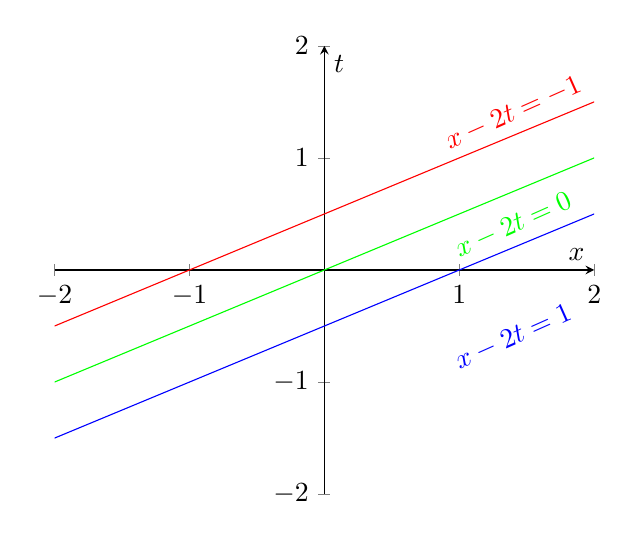
\begin{tikzpicture}
            \begin{axis}[
                    axis lines = middle,
                    xlabel = \(x\),
                    ylabel = \(t\),
                    xmin = -2,
                    xmax = 2,
                    ymin = -2,
                    ymax = 2,
                    xtick distance = 1,
                    ytick distance = 1,
                ]
                \addplot[domain = -2:2, samples = 100, color = red]{x/2 + 0.5};
                \node[rotate = 24, red] at (axis cs: 1.4, 1.4) {\(x - 2t = -1\)};
                \addplot[domain = -2:2, samples = 100, color = green]{x/2 + 0};
                \node[rotate = 24, green] at (axis cs: 1.4, 0.4) {\(x - 2t = 0\)};
                \addplot[domain = -2:2, samples = 100, color = blue]{x/2 - 0.5};
                \node[rotate = 24, blue] at (axis cs: 1.4, -0.6) {\(x - 2t = 1\)};
            \end{axis}
        \end{tikzpicture}
    \end{center}
    We can express \(u(x,y)\) as a function of \(x - 2t\):
    \[u(x, t) = f(x - 2t)\]
    We can solve for \(f\) using the initial condition:
    \[u(x, 0) = f(x) = x^3\]
    Thus, the solution to the transport equation is
    \[u(x, t) = (x - 2t)^3\]
    We can graph \(u(x, 0), u(x, 1), u(x, 2)\) on the same graph:
    \begin{center}
        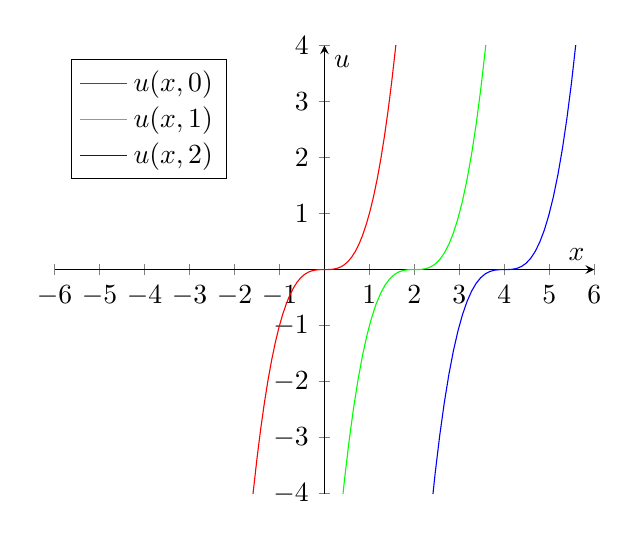
\begin{tikzpicture}
            \begin{axis}[
                    axis lines = middle,
                    xlabel = \(x\),
                    ylabel = \(u\),
                    xmin = -6,
                    xmax = 6,
                    ymin = -4,
                    ymax = 4,
                    xtick distance = 1,
                    ytick distance = 1,
                    legend pos = north west,
                ]
                \addplot[domain = -4:4, samples = 100, color = red]{x^3};
                \addlegendentry{\(u(x, 0)\)}
                \addplot[domain = -4:6, samples = 100, color = green]{(x - 2)^3};
                \addlegendentry{\(u(x, 1)\)}
                \addplot[domain = -4:6, samples = 100, color = blue]{(x - 4)^3};
                \addlegendentry{\(u(x, 2)\)}
            \end{axis}
        \end{tikzpicture}
    \end{center}
    We can see that the solutions are moving to the right with speed 2.
\end{solution}

\pagebreak

\begin{problem}
We define
\[u(x,t) := \frac{1}{\sqrt{4\pi Dt}}e^{-\frac{x^2}{4Dt}}\]
Verify that the function \(u(x,t)\) is a solution of the heat equation
\[u_t = Du_{xx}\]
for all \((x, t)\) with \(-\infty < x < \infty\) and \(t > 0\).
\end{problem}
\begin{solution}
    \begin{align*}
        u_t    & = \frac{1}{\sqrt{4\pi D}}\left(-\frac{1}{2}t^{-\frac{3}{2}}e^{-\frac{x^2}{4Dt}} + t^{-\frac{1}{2}} e^{-\frac{x^2}{4Dt}}\frac{x^2}{4Dt}\right) \\
               & = \frac{1}{2t\sqrt{4\pi Dt}}e^{-\frac{x^2}{4Dt}}\left(\frac{x^2}{2Dt}-1\right)                                                                \\
               & = \frac{1}{2t}\left(\frac{x^2}{2Dt}-1\right) u(x, t)                                                                                          \\
        u_x    & = \frac{1}{\sqrt{4\pi Dt}}e^{-\frac{x^2}{4Dt}}\left(-\frac{x}{2Dt}\right)                                                                     \\
        u_{xx} & = \frac{1}{\sqrt{4\pi Dt}}e^{-\frac{x^2}{4Dt}}\left(\frac{x^2}{4D^2t^2} - \frac{1}{2Dt}\right)                                                \\
               & = \frac{1}{2t\sqrt{4\pi Dt}}e^{-\frac{x^2}{4Dt}}\left(\frac{x^2}{2Dt}-1\right)  \frac{1}{D}                                                   \\
               & = \frac{1}{2Dt}\left(\frac{x^2}{2Dt}-1\right) u(x, t)
    \end{align*}
    We can see that
    \[u_t = Du_{xx}\]
    for all \((x, t)\) with \(-\infty < x < \infty\) and \(t > 0\).
\end{solution}

\pagebreak

\begin{problem}
For \(Q > 0\), compute
\[\int_{-\infty}^{\infty} e^{-Qx^2}dx\]
Hint: Multiply by the identical integral but replace x variable to y, and change vari- ables to polar coordinates.
\end{problem}
\begin{solution}
    Let \(I = \int_{-\infty}^{\infty} e^{-Qx^2}dx = \int_{-\infty}^{\infty} e^{-Qy^2}dy\). Then
    \begin{align*}
        I^2 & = \left(\int_{-\infty}^{\infty} e^{-Qx^2}dx\right)\left(\int_{-\infty}^{\infty} e^{-Qy^2}dy\right) \\
            & = \int_{-\infty}^{\infty}\int_{-\infty}^{\infty} e^{-Q(x^2 + y^2)}dxdy
    \end{align*}
    We can change variables to polar coordinates:
    \begin{align*}
        I^2 & = \int_{0}^{2\pi}\int_{0}^{\infty} e^{-Qr^2}rdrd\theta \\
            & = 2\pi\int_{0}^{\infty} e^{-Qr^2}rdr
    \end{align*}
    Let \(u = -Qr^2\), then \(du = -2Qrdr\). Thus,
    \begin{align*}
        I^2 & = 2\pi\left[\frac{1}{-2Q}e^{-Qr^2}\right]_0^{\infty} \\
            & = \frac{\pi}{Q}
    \end{align*}
    Thus,
    \[I = \int_{-\infty}^{\infty} e^{-Qx^2}dx = \sqrt{\frac{\pi}{Q}}\]
\end{solution}

\pagebreak

\begin{problem}
We will derive the transport equation \(u_t + cu_x = 0\) for \(x, t \in \mathbb{R}\) using an approach via compartment models similar to what we used for the derivation of the heat equation in class: assume that \(u(x, t)\) is the concentration of particles at position \(x\) and time \(t\). Let \(h\) and \(\tau\) be positive and small. First, divide up the real line into intervals of length \(h\) centered at positions \(\hdots, x-2h, x-h, x, x+h, x+2h, \hdots\). Next, we assume that during the time interval from \(t\) to \(t + \tau\) all particles in an interval move to the nearest interval to their right.
\begin{enumerate}[label = (\alph*)]
    \item Write down a balance equation that reflects this situation. Please provide a clear description of the various terms in the balance equation.
    \item Rearrange the terms in your balance equation and substitute them from Taylor expansions appropriately.
    \item Choose an appropriate way to let \(h, t\) go to zero, and show that the limit is the transport equation we want.
\end{enumerate}
\end{problem}
\begin{solution}
    \[\]
    \vspace*{-4em}
    \begin{enumerate}[label = (\alph*)]
        \item Number of particles at time \(t + \tau\) = Number of particles at time \(t\) + Change:
              \[hu(x, t + \tau) = hu(x, t) + \text{Change}\]
              \begin{align*}
                  \text{Change} & = (\text{Number of particles that moved from } x - h \text{ to } x) \\ &\hspace{1em}- (\text{Number of particles that moved from } x \text{ to } x + h). \\
                                & = h\left(u(x - h, t) - u(x, t)\right)
              \end{align*}
              We have
              \[hu(x, t + \tau) = hu(x, t) + h\left(u(x - h, t) - u(x, t)\right)\]
        \item Rearranging the terms and dividing by \(h\tau\), we have
              \begin{equation} \label{eq:1}
                  \frac{u(x, t + \tau) - u(x, t)}{\tau} = \frac{h}{\tau}\,\frac{u(x - h, t) - u(x, t)}{h}
              \end{equation}
              We can use a Taylor expansion to approximate \(u(x - h, t)\)
              \[u(x - h, t) = u(x, t) - hu_x(x, t) + O(h^2)\]
              so that we have
              \[u(x - h, t) - u(x, t) = -hu_x(x, t) + O(h^2)\]
              Substituting into \eqref{eq:1}, we have
              \[\frac{u(x, t + \tau) - u(x, t)}{\tau} = \frac{h}{\tau}\,\frac{-hu_x(x, t) + O(h^2)}{h}\]
              \[\frac{u(x, t + \tau) - u(x, t)}{\tau} = \frac{h}{\tau}\left(-u_x(x, t) + O(h)\right)\]
        \item Let \(h \to 0\) and \(\tau \to 0\). Let us also choose \(\tau = \frac{h}{c}\) so that \(\tau \rightarrow 0\) as \(h \rightarrow 0\). Then
              \[\lim_{h \to 0}\frac{u(x, t + \tau) - u(x, t)}{\tau} = \lim_{h \to 0}\frac{h}{\tau}\left(-u_x(x, t) + O(h)\right)\]
              \[\lim_{\tau \to 0}\frac{u(x, t + \tau) - u(x, t)}{\tau} = \lim_{h \to 0}\frac{h}{\frac{h}{c}}\left(-u_x(x, t) + O(h)\right)\]
              \[u_t(x, t) = -cu_x(x, t)\]
              \[u_t + cu_x = 0\]
              Thus, the limit is the transport equation.
    \end{enumerate}
\end{solution}

\end{document}
